\section{Application I/O benchmark}
\label{sec:app_benchmarks}
In this section, we demonstrate our solution on HACC I/O representing data movement between compute nodes and I/O nodes.

\subsection {HACC I/O}
HACC (Hardware/Hybrid Accelerated Cosmology Code) \cite{Habib:HACC} is a large-scale cosmology code suite that simulates the evolution of the universe through the first 13 billion years after the Big Bang. The simulation tracks the movement of trillions of particles as they collide and interact with each other, forming structure that transform into galaxies. During the runtime, HACC writes data periodically to storage system. The data can also be transferred from Mira to Tukey for data analysis and visualization. In both ways, data needs to go from compute nodes to I/O nodes first. In this benchmark, we use HACC I/O, an I/O benchmark written to evaluate performance of the I/O system for HACC, to show the data transfer performance from compute nodes to I/O nodes by writing to /dev/null. We compare the throughput of our mechanism to default MPI collective write on HACC I/O.
%\subsection{Staging}
%Presenting staging data from Mira to vis cluster Tukey. Analyze the results.

\subsection{Transferring data to I/O nodes}
In this experiments, we scale our experiments from 8,192 up to 131,072 compute cores to simulate the collision of $768^3$ to $2,816^3$ particles. We write only 10\% of the generated data with the amount of 2GB to 85GB of data. The data is written from processes with MPI ranks within the range [4*num\_processes/10, 5*num\_processes/10] with the num\_processes being the total number of MPI ranks in our application. We collect the bandwidth information and report the average. The results are shown in Figure \ref{fig:hacc_agg}

\begin{figure}[!htb]
\vspace{-0.1in}
\centering
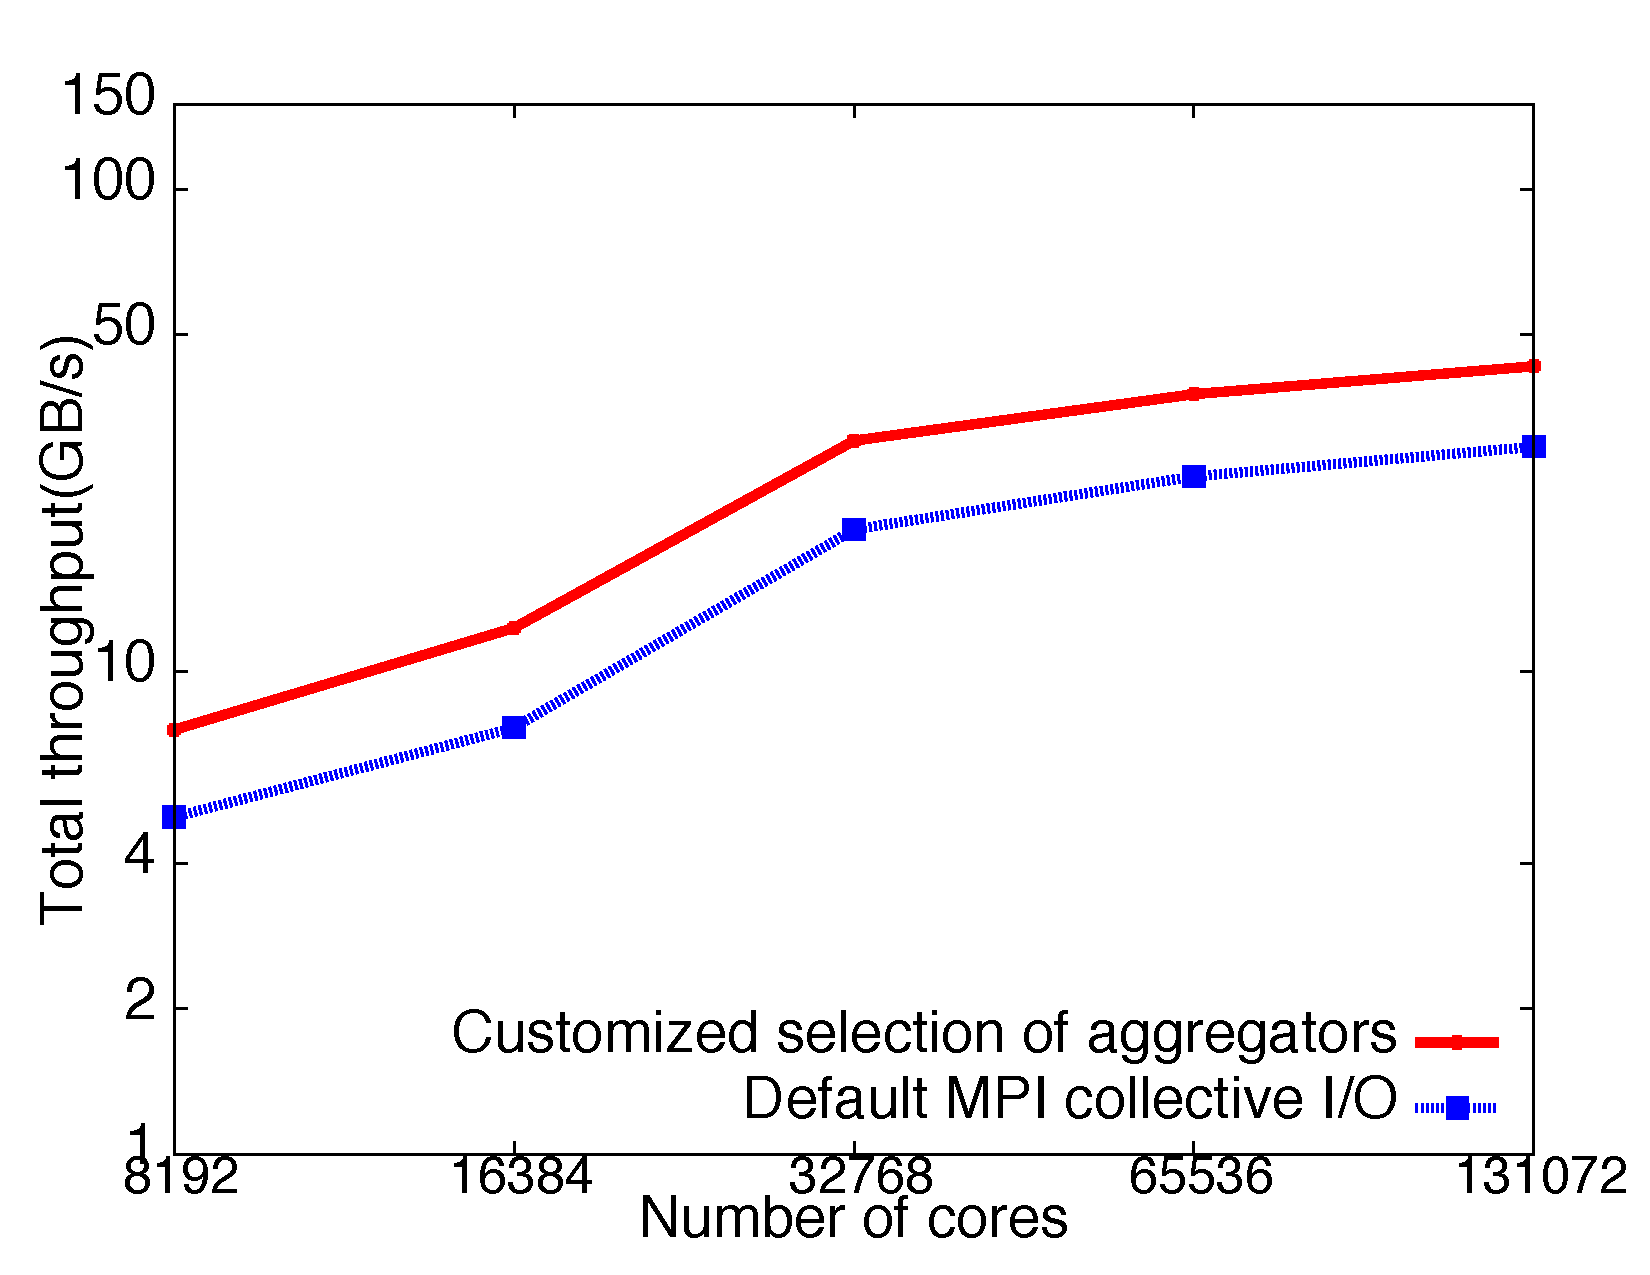
\includegraphics[scale=0.3]{figures/hacc_agg.pdf}
\vspace{-0.1in}
\caption{Write throughput of HACC application to I/O nodes /dev/null}
\vspace{-0.1in}
\label{fig:hacc_agg}
\end{figure}

The results show that in both cases, the number of I/O nodes employed is more than default I/O nodes. However, in our case, the position and location of aggregators are chosen dynamically and are distributed uniformly brought in better performance. Overall we can get up to 50\% throughput improvement. Thus, dynamic selection of number of and location of aggregators based on size of data and interconnect topology is of paramount importance for sparse data movement.

\subsection{Energy consumption comparison}
In these micro-benchmarks, we show that when using multi-path data movement for sparse data patterns, we not only increase bandwidth but also save energy consumption by the system.

\begin{figure}[!htb]
\vspace{-0.1in}
\centering
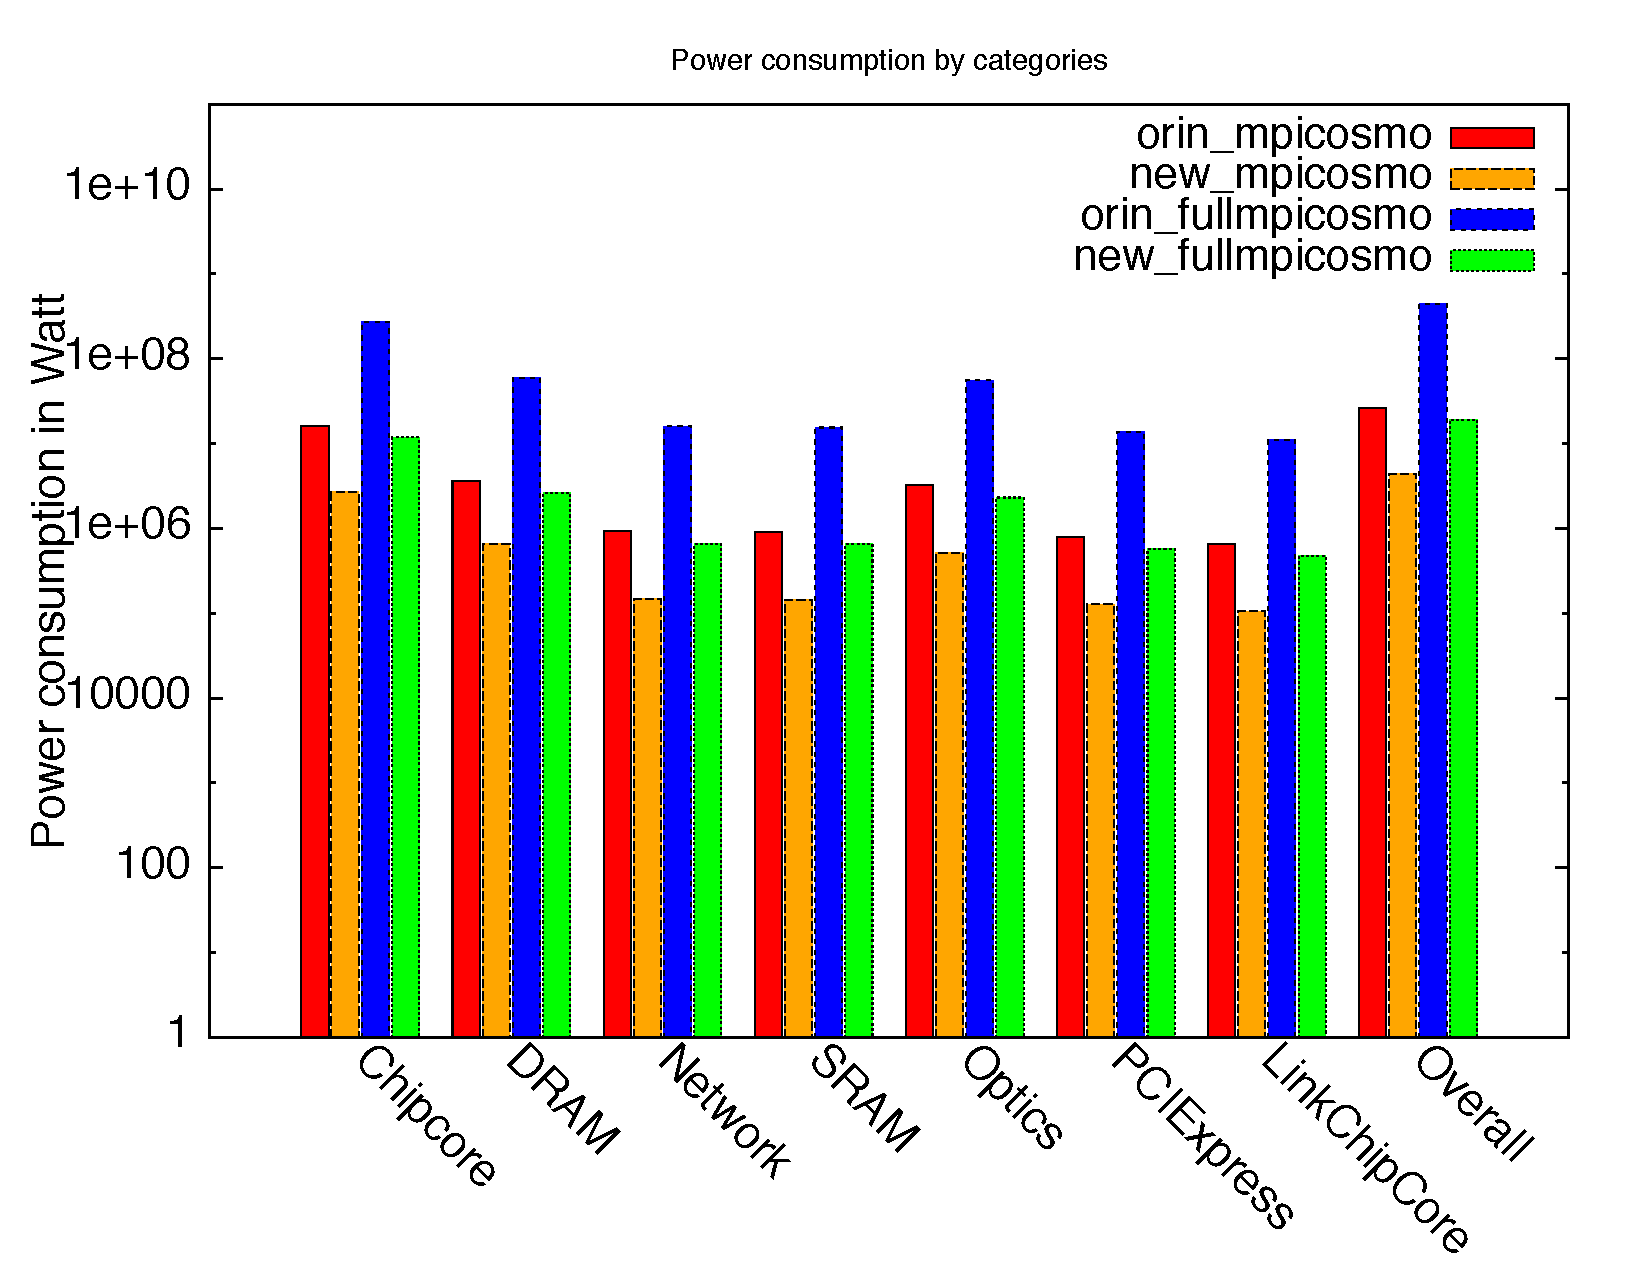
\includegraphics[scale=0.3]{figures/power_cat.pdf}
\vspace{-0.1in}
\caption{Energy consumption by category at a node}
\vspace{-0.1in}
\label{fig:hacc_agg}
\end{figure}

\begin{figure}[!htb]
\vspace{-0.1in}
\centering
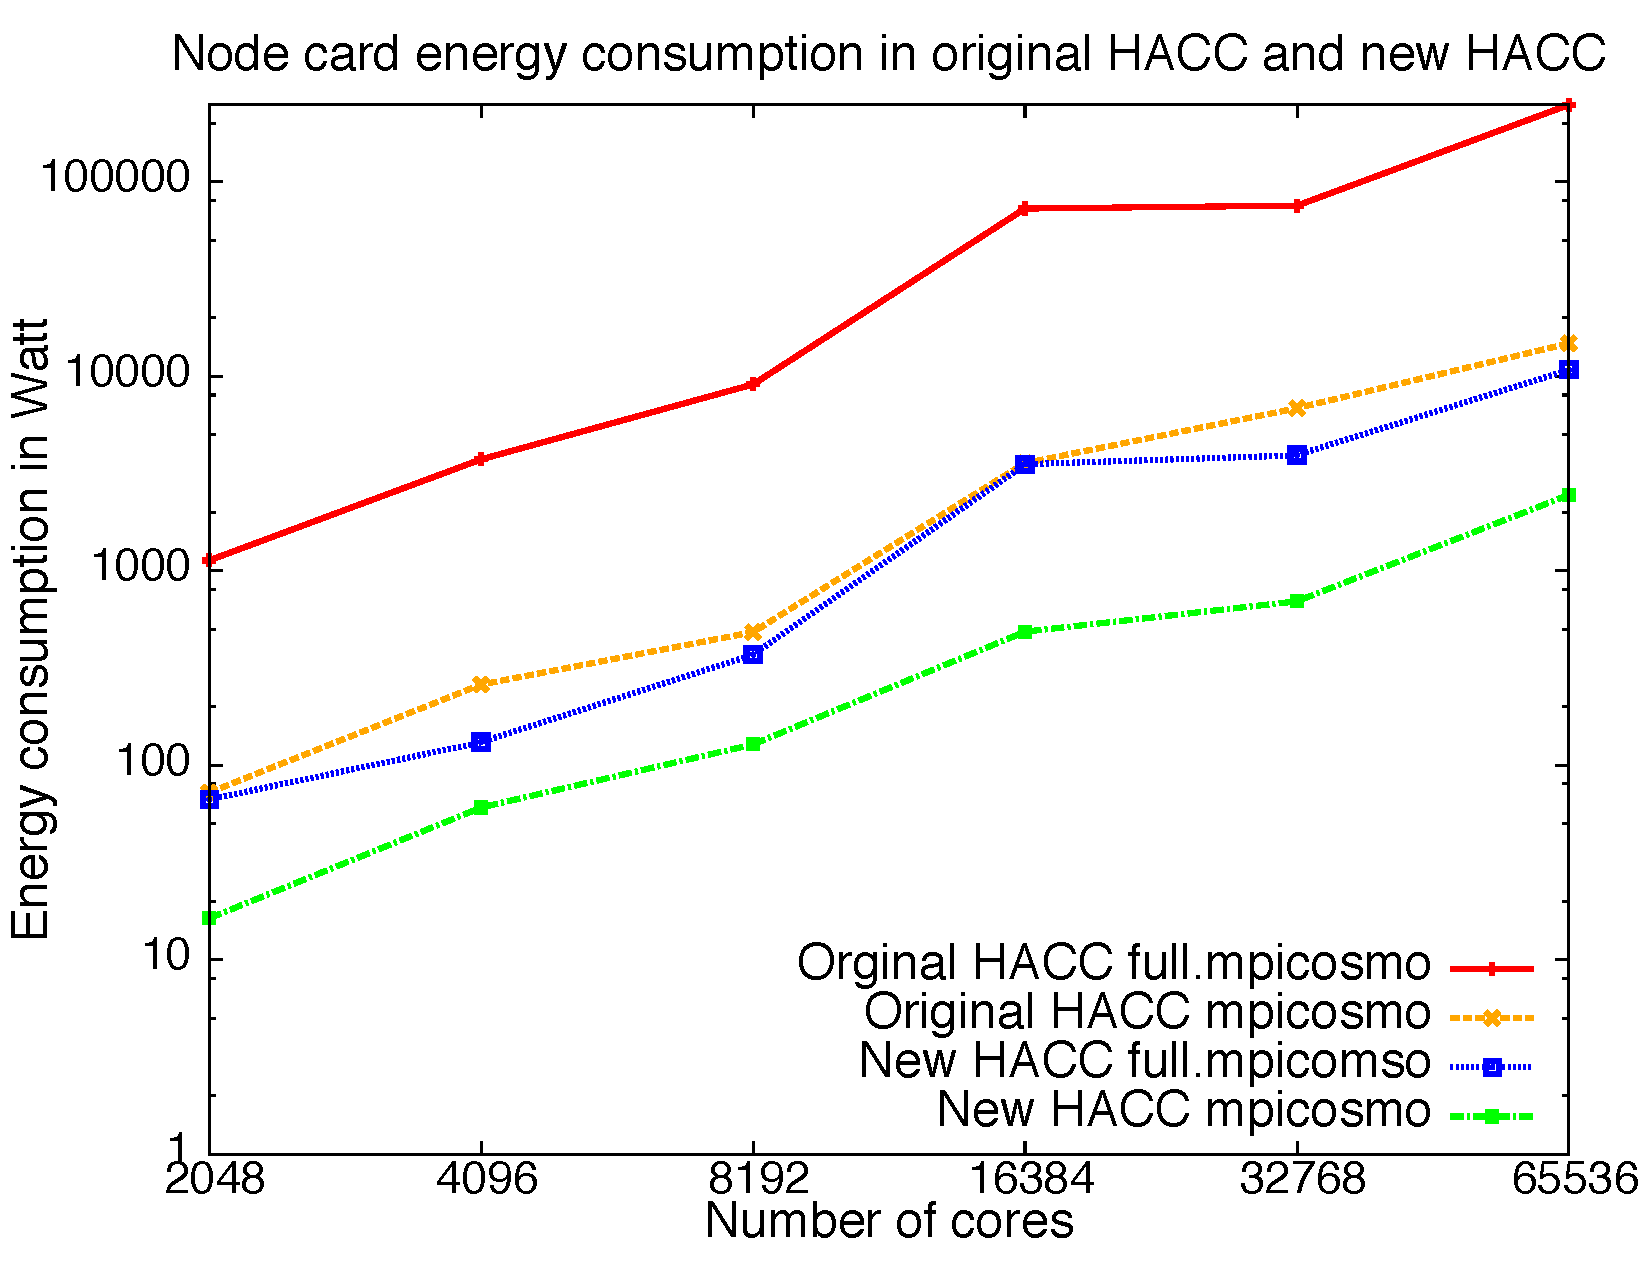
\includegraphics[scale=0.3]{figures/power_ncp.pdf}
\vspace{-0.1in}
\caption{Total energy consumption at scale}
\vspace{-0.1in}
\label{fig:hacc_agg}
\end{figure}
